%experiment
In this chapter, experiment setup will be presented. Any adjustment of from the original architecture implementation also stated in here. Lastly, dataset preprocessing step is explained here. 

\section{Experiment Setup}
All of the experiment is executed on portable computer with specification as follows:
\begin{center}
	\begin{tabular}{| c| c| }
		\hline
		Processor & Intel® Core™ i7 6700HQ Processor\\ 
		\hline
		RAM & 8.0 GB \\  
		\hline
		GPU & NVIDIA® GeForce® GTX 960M \\
		\hline
		VRAM & 2.0 GB     \\
		\hline
	\end{tabular}
\end{center}

For training process, we use Keras with TensorFlow as backend library. Python version that was used is 3.6. For every experiment, we limit it to 10 epochs because the amount to train 1 epoch is quite time consuming for a certain architecture.

\subsection{Architecture Implementation}
Since we are testing on a less powerful machine, we have to adjust the implementation of the architecture as follows.
\subsubsection{LeNet}
There are no adjustment on implementing LeNet from its original version \cite{lecun1998gradient} since the network itself is quite simple and straightforward. The order of the layer as follows: the first layer consists of 6 convolution with filter size of 3x3 and tanh activation function. The second layer consists of MaxPooling layer with a size of 2x2. The third layer is 16 convolution with 2x2 filter size and tanh activation function. The fourth layer is MaxPooling with pool size of 2x2. The fifth layer is flatten layer. The sixth layer is 256 fully-connected layer with tanh activation function. The last layer is 10 fully connected layer with softmax activation function. We use adadelta as the optimizer and categorical cross entropy as the loss. The data was run with 10 epoch and batch size of 128. The code to implement LeNet can be seen on Appendix \ref{code:lenet} and the overview of the architecture design can be seen on \ref{fig:lenet_arch}. All of the codes are available at \href{https://github.com/lightzard/dm-seminar}{https://github.com/lightzard/dm-seminar} .

\begin{figure}[h]
	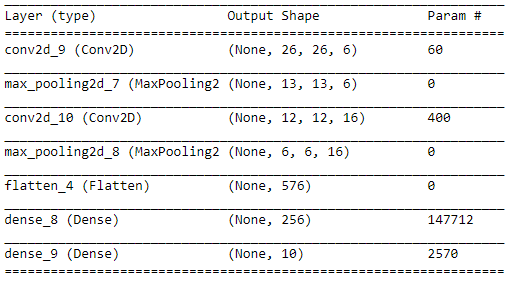
\includegraphics[scale=0.5]{figures/lenet_arch}
	\centering
	\caption{LeNet architecture overview}
	\label{fig:lenet_arch}
\end{figure}

\subsubsection{VGG-Net}
We propose simpler version of VGG-Net because the data is quite small. If we use the original version of VGG, we are running out of input dimension when doing training. Also, implementing original VGG-Net is quite slow and consumes a lot of memory on current machine. The simpler version architecture can bee seen on \ref{fig:vgg_arch} and the code can be seen on Appendix \ref{code:vggnet}. As we can see in the simplified version of VGG-Net, there are only 4 convolutional layer compared to the simplest version of VGG which has 8 convolutional layer. But the design is similar: we have 3x3 filter size in convolutional layer and MaxPool layer in-between convolutional layer. 

\begin{figure}[h]
	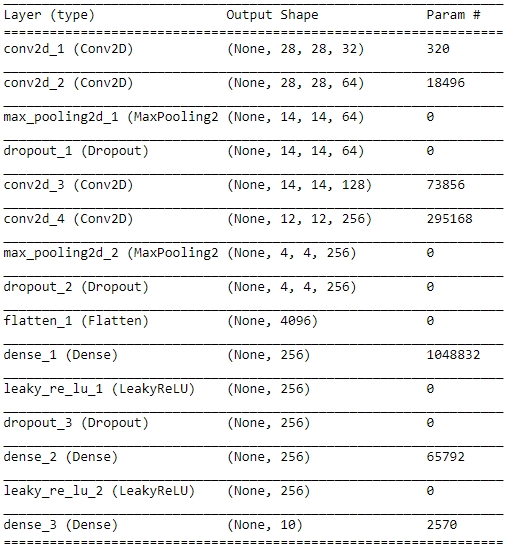
\includegraphics[scale=0.5]{figures/vgg_arch}
	\centering
	\caption{Simpler VGG-Net architecture overview}
	\label{fig:vgg_arch}
\end{figure}

\subsubsection{ResNet V1}
We implement the simplest form of ResNetV1 which is ResNet20V1 due to hardware constraint. In this variation, there are 20 stacks of "resnet block". Each block consists of 2 x (3 x 3) Convolution-Batch Normalization-ReLU layer. 
In applying ResNet, we use ResNet builder library that are available at \href{https://github.com/keras-team/keras/blob/master/examples/cifar10\_resnet.py}{https://github.com/keras-team/keras/blob/master/examples/cifar10\_resnet.py}. Full implementation code can be see at Appendix \ref{code:resnet}.

\subsubsection{ResNet V2}
Implementing ResNet V2 is the same as ResNetV1. We just need to change the parameter of n=2 (so that the depth is equal to 20) and version=2 in the ResNet builder. The difference of ResNet V2 and V1 is that, in V2 each block consists of  (1 x 1)-(3 x 3)-(1 x 1) Batch Normalization-ReLU-Convolution layer. At the beginning of each 'stage', the feature map size is halved (downsampled) by a convolutional layer with strides=2, while the number of filter maps is doubled. Within each 'stage', the layers have the same number filters and the
same filter map sizes.

\subsubsection{AlexNet/SqueezeNet}
Initially we plan to implement AlexNet. But, when we try to implement it on the current machine we failed to implement it because the number of trainable parameters is too big. Then, we discover SqueezeNet \cite{SqueezeNet}, a simpler version of AlexNet that could achieve similar accuracy with less memory resource and training time. The architecture idea can be seen on \ref{fig:squeezenet_arch}. The architecture consists of convoultional layer and fire module. A fire module consists of 1x1 convolutional layer followed by a mix of 1x1 and 3x3 convolution layer. Then, it gradually increase the number of filters per fire module from the beginning to the end of the network. SqueezeNet performs max-pooling with a stride of 2 after layers conv1, fire4, fire8, and conv10.

\begin{figure}[h]
	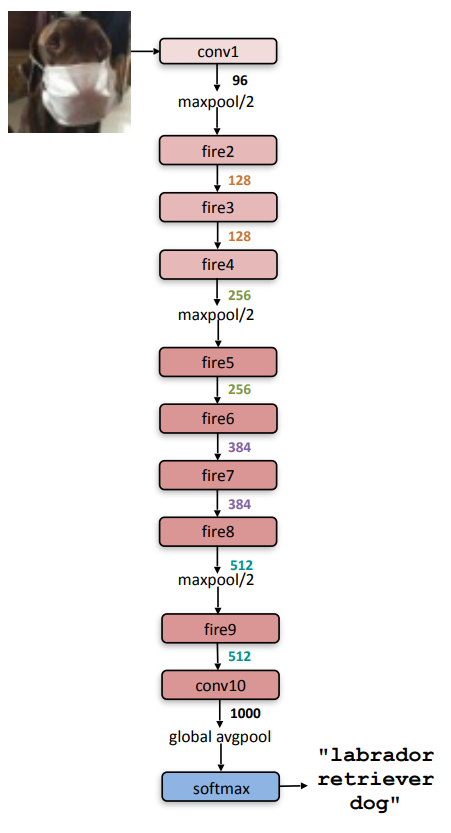
\includegraphics[scale=0.5]{figures/squeezenet}
	\centering
	\caption{SqueezeNet architecture}
	\label{fig:squeezenet_arch}
\end{figure}

This implementation is slight modification from SqueezeNet implementation on MNIST dataset as available on \href{https://github.com/titu1994/Kaggle/blob/master/MNIST/SqueezeNet.py}{https://github.com/titu1994/Kaggle/blob/master/MNIST/SqueezeNet.py}

\subsection{Dataset Preprocessing}
MNIST, Fashion MNIST and CIFAR-10 dataset are available directly from {\tt{keras.datasets}} package. The code to load these 3 datasets can be seen on Appendix \ref{code:mnist}, \ref{code:fashionmnist} and \ref{code:cifar10} respectively. As we can see from these codes, the only pre-processing steps applied for these 3 datasets are reshaping input to (28,28,1) (for MNIST and Fashion-MNIST) and converting classes from numerical type to categorical type. For SVHN dataset, we have to load the data manually and apply preprocessing. First step is to transpose the data. The next step is to rename label '10' to '0' because every '0' images in the dataset is labelled as '10' by default. The next step is to take balanced subsample for training data because the size of the training data is too big. We took 6000 images per class randomly as training data thus we have 60000 images as training data and 26032 testing data since we don't do any sampling on testing data. Full code can be seen on \ref{code:SVHN}



